%!TEX root = main.tex

\section{Dataset} \label{sec:dataset}

An important realization we made during this project is the challenge of working with a real dataset.
Understanding the raw data became a significant portion of the project
Our data comes from golf carts equipped with Lidar and cameras~\cite{Miller16_IROS,Miller17_predictive_ICRA}.
Fortunately, it is relatively straightforward to visualize trajectory data, as opposed to some high-dimensional datasets that exist for other applications. 

% what does raw data look like?
The raw dataset's fields are shown in \cref{table_data}, where (easting,northing) are the latitude/longitude global coordinates, and (x,y) are the coordinates in our global campus map.
Veh id indicates which of the three vehicles corresponds to that data point, or in the pedestrian case, which vehicle sensed that pedestrian.
Ped id is a unique id given to each pedestrian seen.

\begin{figure}
	\centering
	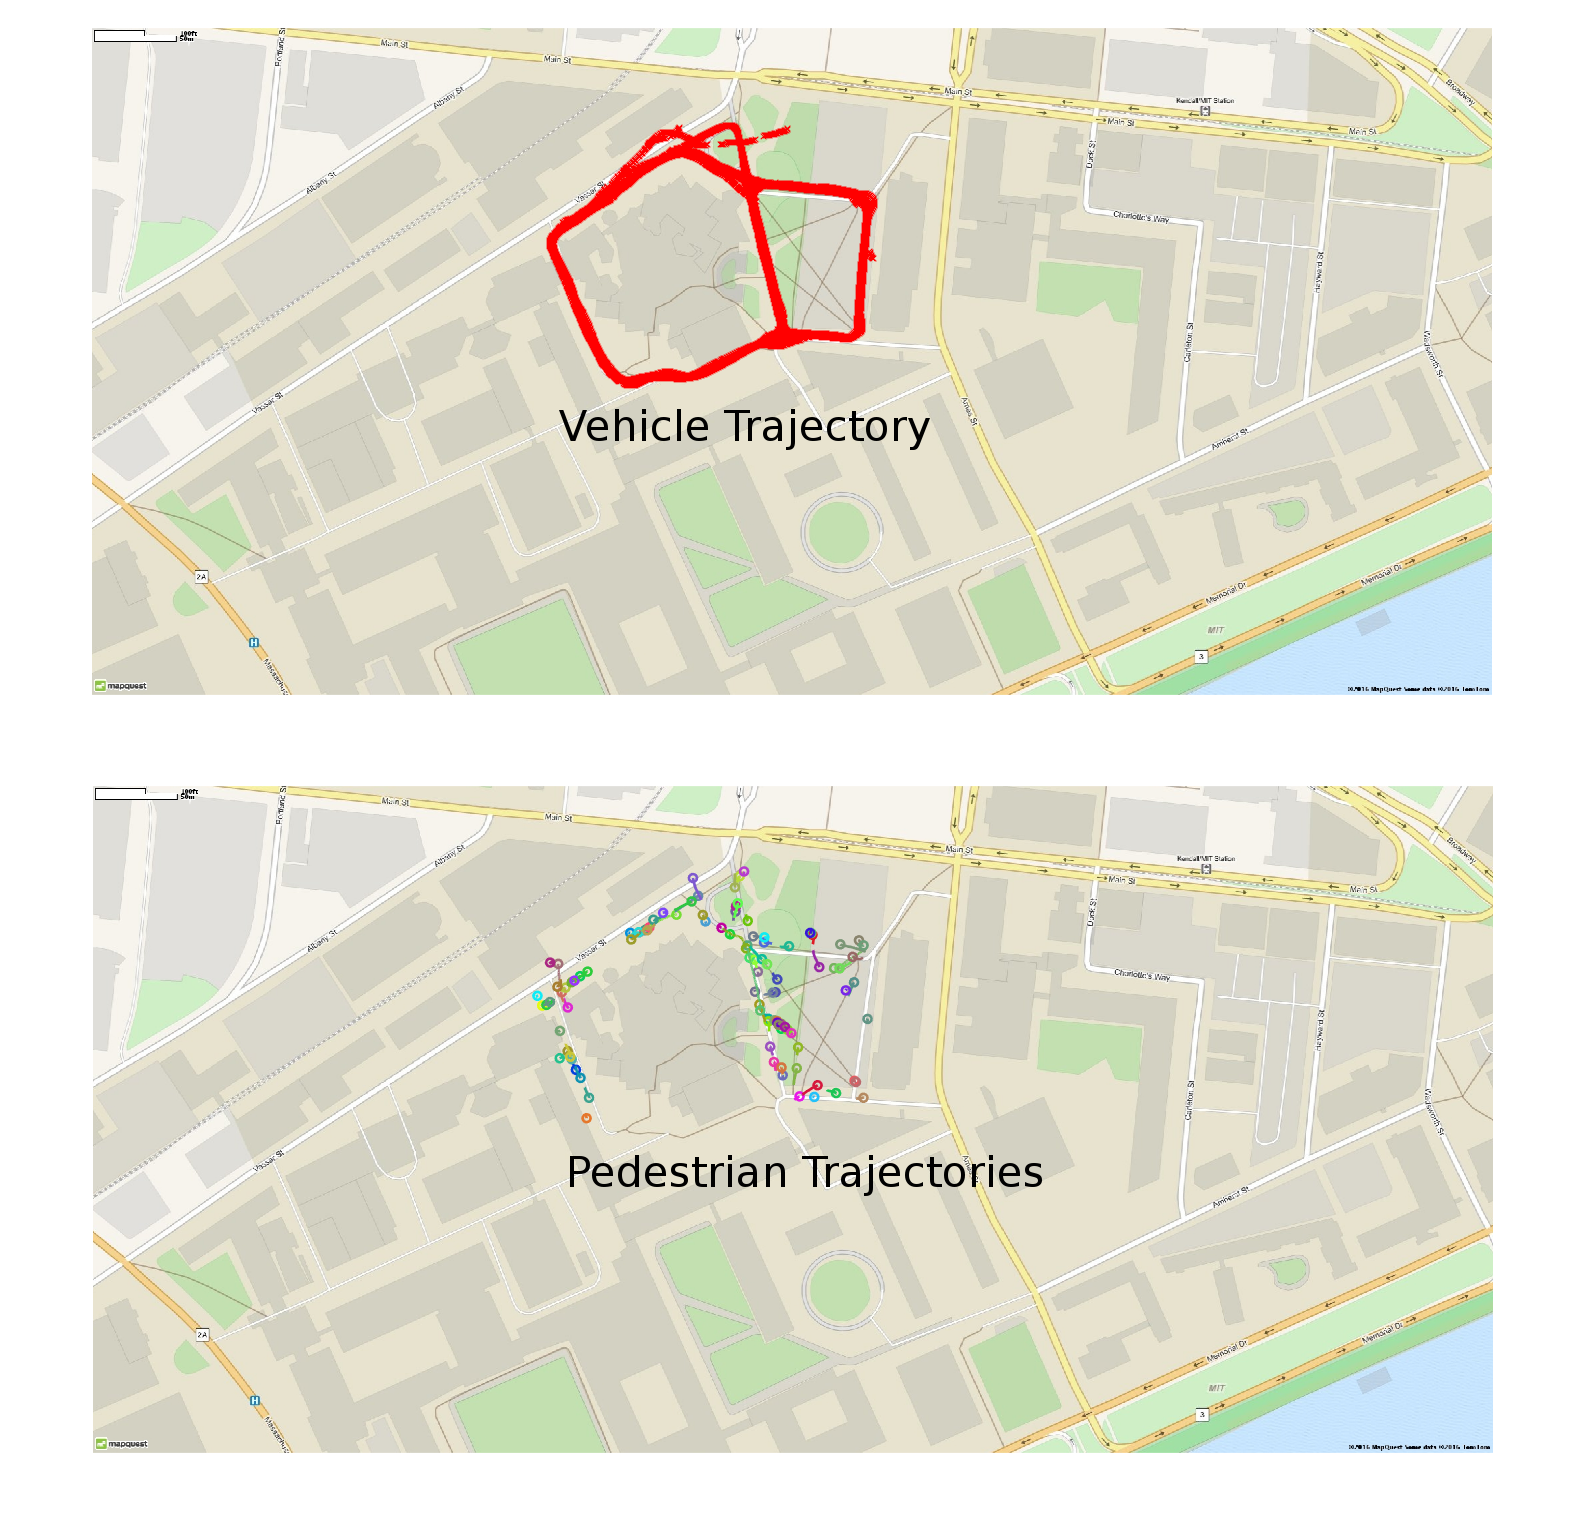
\includegraphics [trim=0 0 0 0, clip, angle=0, width=0.8\columnwidth,
	keepaspectratio]{figures/traj_on_map}
	\caption{The raw trajectories from one day of data collection visualized on a campus map. All trajectories are recorded in the global map coordinate frame.} 
	\label{fig:traj_on_map} 
\end{figure}

\begin{table}[ht!]
\centering
\begin{tabular}{||c||c c c c c c c||}  
 \hline
 \multirow{1}{*}{Type} &
       \multicolumn{7}{c||}{Fields} \\
 \hline\hline
 Vechicle & time & easting & northing & x & y & veh id & \\ \hline
 Pedestrian & time & easting & northing & x & y & veh id & ped id \\ \hline
\end{tabular}
\caption{Raw data fields}
\label{table_data}
\end{table}

% what are the issues with the raw data
There are some noise-related issues with the raw data, as it was collected on a research vehicle under development.
One issue is that the vehicle's (x,y) position sometimes jumps, because the vehicle's localization system does not use GPS and is imperfect.
Other minor issues include pedestrian trajectories that incorrectly split/merge or are too short to be useful for this project.

In addition to addressing noise, we also pre-process the data by converting pedestrian trajectories into the vehicle's local frame.
Specifically for the purpose of our classifier, the pedestrian trajectories must be converted into the vehicle's local frame in order to determine if they cross in front of the vehicle.
That is, our dataset is initially unlabeled, and we must generate the ground truth label that we wish to learn to classify later.

% what is strategy to fix issues
The global-to-local transformation relies on knowledge of vehicle orientation (heading angle) and smooth vehicle trajectories, neither of which we have by default.
\cref{alg:global_to_local} describes the procedure for filtering, transforming, and labeling the raw dataset.

\begin{algorithm}\label{alg:global_to_local}
	\caption{Algorithm for extracting local trajectories}
	\begin{algorithmic}[1]
		\renewcommand{\algorithmicrequire}{\textbf{Input:}}
		\renewcommand{\algorithmicensure}{\textbf{Output:}}
		\REQUIRE $V_g$, $P_g$: global vehicle, pedestrain trajectories~(\cref{table_data})
		\ENSURE  $P_l$: pedestrian trajectories in local vehicle frame
		\FOR {each vehicle}
			\STATE $I_{pos jump}$ = $\{i \in [1,len(V_g)-1] \mid euclid\_dist(V_g(i)-V_g(i+1))>1.0\}$
			\STATE $I_{time jump}$ = $\{i \in [1,len(V_g)-1] \mid time(V_g(i)-V_g(i+1))>0.5\}$
			\STATE J = $I_{pos jump}$ $\cup$ $I_{time jump}$
			\STATE $T_{valid}$ = $\{[J(i), J(i+1)] \mid time(J(i+1) - J(i)) > 5.0\}$
			% \FOR {each segment in $T_{valid}$}
				% \STATE abc
				% \STATE find smooth veh traj
			% % \ENDFOR
			% \FOR {each $P_{g,i}$ pedestrian id}
			% 	\IF {}
			% 		\STATE vxy = 
			% 	\ENDIF
			% \ENDFOR
		\ENDFOR
		\RETURN pedestrian trajectories 
	\end{algorithmic} 
\end{algorithm}

% what does fixed dataset look like



